% Options for packages loaded elsewhere
\PassOptionsToPackage{unicode}{hyperref}
\PassOptionsToPackage{hyphens}{url}
\PassOptionsToPackage{dvipsnames,svgnames,x11names}{xcolor}
%
\documentclass[
]{urban-formatting}

\usepackage{amsmath,amssymb}
\usepackage{iftex}
\ifPDFTeX
  \usepackage[T1]{fontenc}
  \usepackage[utf8]{inputenc}
  \usepackage{textcomp} % provide euro and other symbols
\else % if luatex or xetex
  \usepackage{unicode-math}
  \defaultfontfeatures{Scale=MatchLowercase}
  \defaultfontfeatures[\rmfamily]{Ligatures=TeX,Scale=1}
\fi
\usepackage{lmodern}
\ifPDFTeX\else  
    % xetex/luatex font selection
\fi
% Use upquote if available, for straight quotes in verbatim environments
\IfFileExists{upquote.sty}{\usepackage{upquote}}{}
\IfFileExists{microtype.sty}{% use microtype if available
  \usepackage[]{microtype}
  \UseMicrotypeSet[protrusion]{basicmath} % disable protrusion for tt fonts
}{}
\makeatletter
\@ifundefined{KOMAClassName}{% if non-KOMA class
  \IfFileExists{parskip.sty}{%
    \usepackage{parskip}
  }{% else
    \setlength{\parindent}{0pt}
    \setlength{\parskip}{6pt plus 2pt minus 1pt}}
}{% if KOMA class
  \KOMAoptions{parskip=half}}
\makeatother
\usepackage{xcolor}
\setlength{\emergencystretch}{3em} % prevent overfull lines
\setcounter{secnumdepth}{-\maxdimen} % remove section numbering
% Make \paragraph and \subparagraph free-standing
\ifx\paragraph\undefined\else
  \let\oldparagraph\paragraph
  \renewcommand{\paragraph}[1]{\oldparagraph{#1}\mbox{}}
\fi
\ifx\subparagraph\undefined\else
  \let\oldsubparagraph\subparagraph
  \renewcommand{\subparagraph}[1]{\oldsubparagraph{#1}\mbox{}}
\fi


\providecommand{\tightlist}{%
  \setlength{\itemsep}{0pt}\setlength{\parskip}{0pt}}\usepackage{longtable,booktabs,array}
\usepackage{calc} % for calculating minipage widths
% Correct order of tables after \paragraph or \subparagraph
\usepackage{etoolbox}
\makeatletter
\patchcmd\longtable{\par}{\if@noskipsec\mbox{}\fi\par}{}{}
\makeatother
% Allow footnotes in longtable head/foot
\IfFileExists{footnotehyper.sty}{\usepackage{footnotehyper}}{\usepackage{footnote}}
\makesavenoteenv{longtable}
\usepackage{graphicx}
\makeatletter
\def\maxwidth{\ifdim\Gin@nat@width>\linewidth\linewidth\else\Gin@nat@width\fi}
\def\maxheight{\ifdim\Gin@nat@height>\textheight\textheight\else\Gin@nat@height\fi}
\makeatother
% Scale images if necessary, so that they will not overflow the page
% margins by default, and it is still possible to overwrite the defaults
% using explicit options in \includegraphics[width, height, ...]{}
\setkeys{Gin}{width=\maxwidth,height=\maxheight,keepaspectratio}
% Set default figure placement to htbp
\makeatletter
\def\fps@figure{htbp}
\makeatother

% urban-short-report.tex
% v1.0 Dec. 2021

%\documentclass{urban-formatting}

% Font and Font Weight
\usepackage[default]{lato}
\usepackage[T1]{fontenc}

% Setting the references list
\bibliography{references}

% Change out report title - use shortened title if necessary
\title{REPORT TITLE HERE: USE A SHORTENED TITLE IF NECESSARY}
\makeatletter
\makeatother
\makeatletter
\makeatother
\makeatletter
\@ifpackageloaded{caption}{}{\usepackage{caption}}
\AtBeginDocument{%
\ifdefined\contentsname
  \renewcommand*\contentsname{Table of contents}
\else
  \newcommand\contentsname{Table of contents}
\fi
\ifdefined\listfigurename
  \renewcommand*\listfigurename{List of Figures}
\else
  \newcommand\listfigurename{List of Figures}
\fi
\ifdefined\listtablename
  \renewcommand*\listtablename{List of Tables}
\else
  \newcommand\listtablename{List of Tables}
\fi
\ifdefined\figurename
  \renewcommand*\figurename{Figure}
\else
  \newcommand\figurename{Figure}
\fi
\ifdefined\tablename
  \renewcommand*\tablename{Table}
\else
  \newcommand\tablename{Table}
\fi
}
\@ifpackageloaded{float}{}{\usepackage{float}}
\floatstyle{ruled}
\@ifundefined{c@chapter}{\newfloat{codelisting}{h}{lop}}{\newfloat{codelisting}{h}{lop}[chapter]}
\floatname{codelisting}{Listing}
\newcommand*\listoflistings{\listof{codelisting}{List of Listings}}
\makeatother
\makeatletter
\@ifpackageloaded{caption}{}{\usepackage{caption}}
\@ifpackageloaded{subcaption}{}{\usepackage{subcaption}}
\makeatother
\makeatletter
\@ifpackageloaded{tcolorbox}{}{\usepackage[skins,breakable]{tcolorbox}}
\makeatother
\makeatletter
\@ifundefined{shadecolor}{\definecolor{shadecolor}{rgb}{.97, .97, .97}}
\makeatother
\makeatletter
\makeatother
\makeatletter
\makeatother
\ifLuaTeX
  \usepackage{selnolig}  % disable illegal ligatures
\fi
\IfFileExists{bookmark.sty}{\usepackage{bookmark}}{\usepackage{hyperref}}
\IfFileExists{xurl.sty}{\usepackage{xurl}}{} % add URL line breaks if available
\urlstyle{same} % disable monospaced font for URLs
\hypersetup{
  colorlinks=true,
  linkcolor={blue},
  filecolor={Maroon},
  citecolor={Blue},
  urlcolor={Blue},
  pdfcreator={LaTeX via pandoc}}

\author{}
\date{}

\begin{document}
\ifdefined\Shaded\renewenvironment{Shaded}{\begin{tcolorbox}[interior hidden, frame hidden, breakable, enhanced, borderline west={3pt}{0pt}{shadecolor}, sharp corners, boxrule=0pt]}{\end{tcolorbox}}\fi

\pagenumbering{roman}

\begin{titlepage}
    % Add Policy Center/Intaitive/Toxonmy Term Bar
    % note the textbox exceeds width of document to avoid white space on sides
    \begin{textblock*}{9in}(-0.25in, 0.15in)
        \begin{tcolorbox}[valign = center]
            \begin{center}
                \policycenter{Research Methods and Data Analytics}
            \end{center}
        \end{tcolorbox}
    \end{textblock*}

    % Adding the cover image - code forces the image to be width of full paper (ignoring margins)
    \vspace*{-1.7cm}
    \noindent
    \makebox[\textwidth]{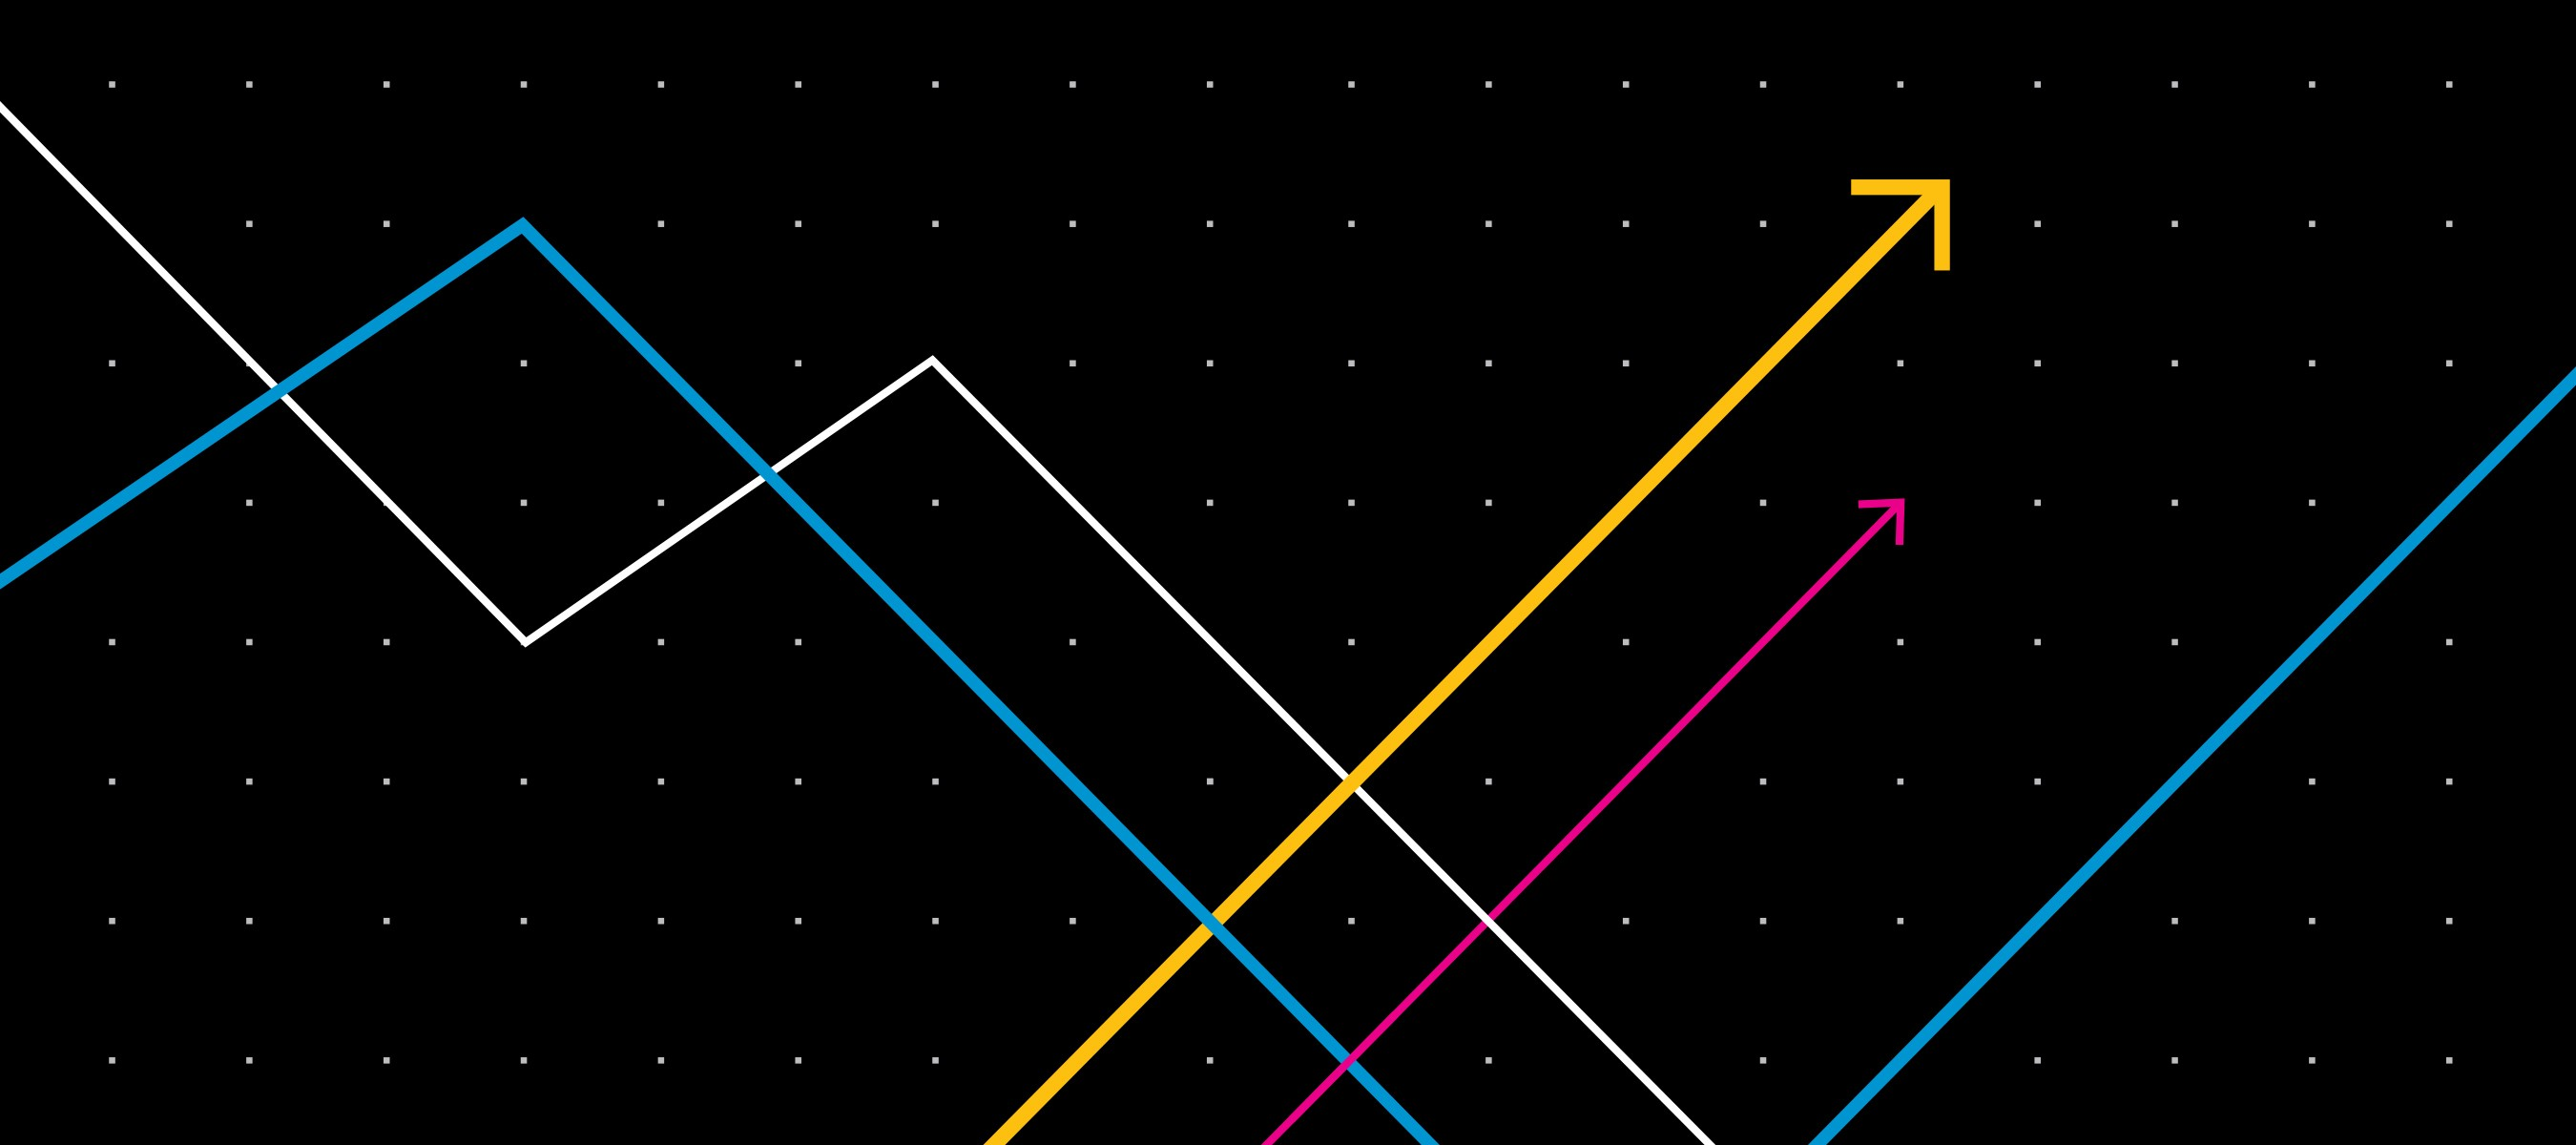
\includegraphics{images/cover.jpg}}
    
    \vspace{0.35in}
    \noindent\textcolor{urban-blue}{\MakeUppercase{\textbf{Research Report}}}
    
    \titlereport{Opt-In Statistical Disclosure Protections}
    
    \vspace{-0.25in}
    
    \reportsubtitle{Empowering Survey Respondents to Improve Data Quality}
    % Multiple column author names - change the "4" to the number of desired columns
    \begin{multicols}{4}
        \authorfont{Aaron R. Williams}
        
        \authorfont{Jen Andre}
      
    \end{multicols}
    
    \vspace{-0.75cm}
    
    \datefont{August 2023}

    % Add logo
    \begin{textblock*}{4.5in}[1, 1](5.5in, 10.5in)
        \noindent
\includegraphics[width=4.5in]{images/cover-footer.jpg}
    \end{textblock*}
\end{titlepage}

%%%%%%%%%%%%%%%%%%%%%%%%%%%%%%%%%%%% About Urban %%%%%%%%%%%%%%%%%%%%%%%%%%%%%%%%%%%
\thispagestyle{empty} % Removed Page Number
\begin{figure}
    
\includegraphics[width=1.5in]{images/logo.png}
\end{figure}
\vspace*{-0.5in}
\about{About the Urban Institute}\\
\vspace{-5pt}
\boilerplate{The nonprofit Urban Institute is a leading research organization dedicated to developing evidence-based insights that improve people’s lives and strengthen communities. For 50 years, Urban has been the trusted source for rigorous analysis of complex social and economic issues; strategic advice to policymakers, philanthropists, and practitioners; and new, promising ideas that expand opportunities for all. Our work inspires effective decisions that advance fairness and enhance the well-being of people and places.}

\vspace*{\fill}
\begin{singlespace}
    \noindent Copyright ©\tbf{Month Year}. Urban Institute. Permission is granted for reproduction of this file, with attribution to the Urban Institute. Cover image by \tbf{Tim Meko}.
\end{singlespace}

\cleardoublepage

\setcounter{page}{3}
\begin{singlespace}
    \tableofcontents
\end{singlespace}

\thispagestyle{empty}

% Footer Formatting: DO NOT CHANGE -----------------------------------
\fancyfoot{}

\fancyfoot[LE]{\colorbox{urban-footergray}{\makebox(0.2, 0.12)[r]{\fontsize{7.5}{0}\selectfont\bfseries{\MakeUppercase{}\hspace{0.2in}}}}\colorbox{urban-gold}{\makebox(0.2, 0.12)[c]{\fontsize{7.5}{0}\selectfont\bfseries{\MakeUppercase\thepage}}}\colorbox{urban-footergray}{\makebox(5.64, 0.12)[r]{\fontsize{7.5}{0}\selectfont\bfseries{\MakeUppercase{Acknowledgments}\hspace{0.2in}}}}}

\fancyfoot[RO]{\colorbox{urban-footergray}{\makebox(5.64, 0.12)[l]{\fontsize{7.5}{0}\selectfont\bfseries{\hspace{0.2in}\MakeUppercase{Acknowledgments}}}}\colorbox{urban-gold}{\makebox(0.2, 0.12)[c]{\fontsize{7.5}{0}\selectfont\bfseries{\MakeUppercase\thepage}}}\colorbox{urban-footergray}{\makebox(0.2, 0.12)[r]{\fontsize{7.5}{0}\selectfont\bfseries{\MakeUppercase{}\hspace{0.2in}}}}}
% Footer Formatting: DO NOT CHANGE -----------------------------------
%%%%%%%%%%%%%%%%%%%%%%%%%%%%%%%%%%%% Acknowledgments %%%%%%%%%%%%%%%%%%%%%%%%%%%%%%%%%%%%
\part{Acknowledgments}

This report was funded by \tbf{[insert your funder name(s) here].} We are grateful to them and to all our funders, who make it possible for Urban to advance its mission. 

The views expressed are those of the \tbf{author/authors} and should not be attributed to the Urban Institute, its trustees, or its funders. Funders do not determine research findings or the insights and recommendations of Urban experts. Further information on the Urban Institute’s funding principles is available at \textcolor{urban-url}{urban.org/fundingprinciples}.

\tbf{[Add any other thanks and contract details here. It may be appropriate to also acknowledge your funder’s funder(s). When in doubt, please check with your center director and Contracts.]}

% Footer Formatting: DO NOT CHANGE -----------------------------------
\fancyfoot{}

\fancyfoot[LE]{\colorbox{urban-footergray}{\makebox(0.2, 0.12)[r]{\fontsize{7.5}{0}\selectfont\bfseries{\MakeUppercase{}\hspace{0.2in}}}}\colorbox{urban-gold}{\makebox(0.2, 0.12)[c]{\fontsize{7.5}{0}\selectfont\bfseries{\MakeUppercase\thepage}}}\colorbox{urban-footergray}{\makebox(5.64, 0.12)[r]{\fontsize{7.5}{0}\selectfont\bfseries{\MakeUppercase{Executive Summary}\hspace{0.2in}}}}}

\fancyfoot[RO]{\colorbox{urban-footergray}{\makebox(5.64, 0.12)[l]{\fontsize{7.5}{0}\selectfont\bfseries{\hspace{0.2in}\MakeUppercase{Executive Summary}}}}\colorbox{urban-gold}{\makebox(0.2, 0.12)[c]{\fontsize{7.5}{0}\selectfont\bfseries{\MakeUppercase\thepage}}}\colorbox{urban-footergray}{\makebox(0.2, 0.12)[r]{\fontsize{7.5}{0}\selectfont\bfseries{\MakeUppercase{}\hspace{0.2in}}}}}
% Footer Formatting: DO NOT CHANGE -----------------------------------
%%%%%%%%%%%%%%%%%%%%%%%%%%%%%%%%%%%% Executive %%%%%%%%%%%%%%%%%%%%%%%%%%%%%%%%%%%%%%%%%
\part{Executive Summary}

\intropara{Body Text style or Chapter Intro Para style here (text shown is in Chapter Intro Para). If you do not have an executive summary, remove this section.}

\section{First-Level Heading in Title Case (Heading 2 style)}

Body Text style for first paragraph under a heading.

Body Text First Indent style for all subsequent paragraphs. \tbf{To add an endnote, use the Insert Endnote function. Endnotes will automatically appear in the Notes section after the appendixes.}\endnote{Endnotes should appear automatically under the Notes heading. If they’re showing up somewhere else, ask your editor or your center’s Word expert for assistance.}

\subsection{Second-Level Heading in Title Case (Heading 3 style)}

Body Text style for first paragraph under a heading.

Body Text First Indent style for all subsequent paragraphs.


\subsubsection{Third-level heading; all caps is built into style (heading 4 style)}

Body Text style for first paragraph under a heading.

Body Text First Indent style for all subsequent paragraphs.

\part{Opt-In Statistical Disclosure Protections}

\section{Introduction}

\section{Methods}

\subsection{Local Differential Privacy}

\subsection{Modeling Opt-In Decisions}

\section{Results}

\section{Conclusion}

% Footer Formatting: DO NOT CHANGE -----------------------------------
\fancyfoot{}

\fancyfoot[LE]{\colorbox{urban-footergray}{\makebox(0.2, 0.12)[r]{\fontsize{7.5}{0}\selectfont\bfseries{\MakeUppercase{}\hspace{0.2in}}}}\colorbox{urban-gold}{\makebox(0.2, 0.12)[c]{\fontsize{7.5}{0}\selectfont\bfseries{\MakeUppercase\thepage}}}\colorbox{urban-footergray}{\makebox(5.64, 0.12)[r]{\fontsize{7.5}{0}\selectfont\bfseries{\MakeUppercase{Appendix}\hspace{0.2in}}}}}

\fancyfoot[RO]{\colorbox{urban-footergray}{\makebox(5.64, 0.12)[l]{\fontsize{7.5}{0}\selectfont\bfseries{\hspace{0.2in}\MakeUppercase{Appendix}}}}\colorbox{urban-gold}{\makebox(0.2, 0.12)[c]{\fontsize{7.5}{0}\selectfont\bfseries{\MakeUppercase\thepage}}}\colorbox{urban-footergray}{\makebox(0.2, 0.12)[r]{\fontsize{7.5}{0}\selectfont\bfseries{\MakeUppercase{}\hspace{0.2in}}}}}
% Footer Formatting: DO NOT CHANGE -----------------------------------
%%%%%%%%%%%%%%%%%%%%%%%%%%%%%%%%%%%% Appendix %%%%%%%%%%%%%%%%%%%%%%%%%%%%%%%%%%%%%%%%%%%
\begin{FlushLeft}
    \part{Appendix Letter. Appendix Title in Title Case}
\end{FlushLeft}

Use the same text styles you used in the main report.

% Footer Formatting: DO NOT CHANGE -----------------------------------
\fancyfoot{}

\fancyfoot[LE]{\colorbox{urban-footergray}{\makebox(0.2, 0.12)[r]{\fontsize{7.5}{0}\selectfont\bfseries{\MakeUppercase{}\hspace{0.2in}}}}\colorbox{urban-gold}{\makebox(0.2, 0.12)[c]{\fontsize{7.5}{0}\selectfont\bfseries{\MakeUppercase\thepage}}}\colorbox{urban-footergray}{\makebox(5.64, 0.12)[r]{\fontsize{7.5}{0}\selectfont\bfseries{\MakeUppercase{Notes}\hspace{0.2in}}}}}

\fancyfoot[RO]{\colorbox{urban-footergray}{\makebox(5.64, 0.12)[l]{\fontsize{7.5}{0}\selectfont\bfseries{\hspace{0.2in}\MakeUppercase{Notes}}}}\colorbox{urban-gold}{\makebox(0.2, 0.12)[c]{\fontsize{7.5}{0}\selectfont\bfseries{\MakeUppercase\thepage}}}\colorbox{urban-footergray}{\makebox(0.2, 0.12)[r]{\fontsize{7.5}{0}\selectfont\bfseries{\MakeUppercase{}\hspace{0.2in}}}}}

% Notes Title Formatting
\renewcommand\notesname{\color{urban-blue}\fontsize{28}{0pt}\selectfont Notes\vspace{-12pt}}
% Footer Formatting: DO NOT CHANGE -----------------------------------

%%%%%%%%%%%%%%%%%%%%%%%%%%%%%%%%%%%% Notes %%%%%%%%%%%%%%%%%%%%%%%%%%%%%%%%%%%%%%%%%%%%%%
\addcontentsline{toc}{part}{Notes}
\theendnotes

% Footer Formatting: DO NOT CHANGE -----------------------------------
\fancyfoot{}

\fancyfoot[LE]{\colorbox{urban-footergray}{\makebox(0.2, 0.12)[r]{\fontsize{7.5}{0}\selectfont\bfseries{\MakeUppercase{}\hspace{0.2in}}}}\colorbox{urban-gold}{\makebox(0.2, 0.12)[c]{\fontsize{7.5}{0}\selectfont\bfseries{\MakeUppercase\thepage}}}\colorbox{urban-footergray}{\makebox(5.64, 0.12)[r]{\fontsize{7.5}{0}\selectfont\bfseries{\MakeUppercase{References}\hspace{0.2in}}}}}

\fancyfoot[RO]{\colorbox{urban-footergray}{\makebox(5.64, 0.12)[l]{\fontsize{7.5}{0}\selectfont\bfseries{\hspace{0.2in}\MakeUppercase{References}}}}\colorbox{urban-gold}{\makebox(0.2, 0.12)[c]{\fontsize{7.5}{0}\selectfont\bfseries{\MakeUppercase\thepage}}}\colorbox{urban-footergray}{\makebox(0.2, 0.12)[r]{\fontsize{7.5}{0}\selectfont\bfseries{\MakeUppercase{}\hspace{0.2in}}}}}
% Footer Formatting: DO NOT CHANGE -----------------------------------
%%%%%%%%%%%%%%%%%%%%%%%%%%%%%%%%%%%% References %%%%%%%%%%%%%%%%%%%%%%%%%%%%%%%%%%%%%%%%%
\addcontentsline{toc}{part}{References}

\printbibliography[title={\color{urban-blue}\fontsize{28}{18}\selectfont References}]

% Footer Formatting: DO NOT CHANGE -----------------------------------
\fancyfoot{}

\fancyfoot[LE]{\colorbox{urban-footergray}{\makebox(0.2, 0.12)[r]{\fontsize{7.5}{0}\selectfont\bfseries{\MakeUppercase{}\hspace{0.2in}}}}\colorbox{urban-gold}{\makebox(0.2, 0.12)[c]{\fontsize{7.5}{0}\selectfont\bfseries{\MakeUppercase\thepage}}}\colorbox{urban-footergray}{\makebox(5.64, 0.12)[r]{\fontsize{7.5}{0}\selectfont\bfseries{\MakeUppercase{About the Authors}\hspace{0.2in}}}}}

\fancyfoot[RO]{\colorbox{urban-footergray}{\makebox(5.64, 0.12)[l]{\fontsize{7.5}{0}\selectfont\bfseries{\hspace{0.2in}\MakeUppercase{About the Authors}}}}\colorbox{urban-gold}{\makebox(0.2, 0.12)[c]{\fontsize{7.5}{0}\selectfont\bfseries{\MakeUppercase\thepage}}}\colorbox{urban-footergray}{\makebox(0.2, 0.12)[r]{\fontsize{7.5}{0}\selectfont\bfseries{\MakeUppercase{}\hspace{0.2in}}}}}
% Footer Formatting: DO NOT CHANGE -----------------------------------
%%%%%%%%%%%%%%%%%%%%%%%%%%%%%%%%%%%% About Author %%%%%%%%%%%%%%%%%%%%%%%%%%%%%%%%%%%%%%
\part{About the Authors}

\textbf{Aaron R. Williams} but the rest of the text lightface. Use Author Bios--First style for the introductory paragraph of each bio. You can paste your bio from your author page on the Urban website (and condense it if needed) here.\\
If your bio is more than one paragraph long, use Author Bios--Additional for any subsequent paragraphs. This style suppresses spacing between paragraphs.\\
Author bios no longer include photos.

\noindent\textbf{Jennifer Andre} but the rest of the text lightface. Use Author Bios--First style for the introductory paragraph of each bio. You can paste your bio from your author page on the Urban website (and condense it if needed) here.\\
If your bio is more than one paragraph long, use Author Bios--Additional for any subsequent paragraphs. This style suppresses spacing between paragraphs.\\
Author bios no longer include photos.

%%%%%%%%%%%%%%%%%%%%%%%%%%%%%%%%%%%% Statement of Independence %%%%%%%%%%%%%%%%%%%%%%%%%%
\addcontentsline{toc}{part}{Statement of Independence}
\thispagestyle{empty} 

\about{S\scalebox{0.8}{tatement of} I\scalebox{0.8}{ndependence}}
\vspace{-5pt}
\boilerplate{The Urban Institute strives to meet the highest standards of integrity and quality in its research and analyses and in the evidence-based policy recommendations offered by its researchers and experts. We believe that operating consistent with the values of independence, rigor, and transparency is essential to maintaining those standards. As an organization, the Urban Institute does not take positions on issues, but it does empower and support its experts in sharing their own evidence-based views and policy recommendations that have been shaped by scholarship. Funders do not determine our research findings or the insights and recommendations of our experts. Urban scholars and experts are expected to be objective and follow the evidence wherever it may lead.}

\newpage
\thispagestyle{empty}

\begin{textblock*}{8.5in}[1, 1](8.5in, 11in)
    \noindent
\includegraphics[width=\paperwidth,height=\paperheight]{images/back.pdf}
\end{textblock*}



\newpage
\thispagestyle{empty}

\begin{textblock*}{8.5in}[1, 1](8.5in, 11in)
    \noindent
\includegraphics[width=\paperwidth,height=\paperheight]{images/back.pdf}
\end{textblock*}

\end{document}

\end{document}
